\documentclass{tufte-handout}
\usepackage{tikz}\usetikzlibrary{decorations.pathreplacing,positioning,chains}
\usepackage{tipa}
\usepackage{color}
\usepackage{listings}
\usepackage{amsmath}
\usepackage{booktabs}

\input{vc.tex}


\usepackage[lastexercise,answerdelayed]{exercise}
\setlength{\Exesep}{.5ex}
\setlength{\Exetopsep}{1em}
\renewcommand{\ExerciseListName}{Exercise}
\renewcommand{\AnswerListName}{}
\renewcommand{\ExerciseHeaderTitle}{(\emph{\ExerciseTitle.})\ }
\renewcommand{\ExerciseListHeader}{\ExerciseHeaderDifficulty%
\textbf{\ExerciseListName\ExerciseHeaderNB.}\ \ExerciseHeaderTitle%
\ExerciseHeaderOrigin\ignorespaces}
\renewcommand{\AnswerListHeader}{\textbf{\ExerciseHeaderNB.\ }}

\title{Amortised analysis}
\author{Thore Husfeldt}
\date{\small Revision {\tt \GITAbrHash}$\ldots$, \GITAuthorDate, \GITAuthorName}
\begin{document}
\maketitle
\begin{abstract}
  This note covers the technique of amortized analysis, as a
  supplement to [SW], the textbook \emph{Algorithms, 4th ed.} by
  Sedgewick and Wayne.

  It contains a complete answer to exercise 1.4.32 thus completing the
  proof of proposition~E in section 1.4.
\end{abstract}

\section{Resizing array}
\label{sec-1.1}

Consider the resizing array implementation of {\tt Stack} (Algorithm
1.1) and the collowing claim:

   
\begin{quote} {\bf Proposition A1.} In the resizing array
  implementation of {\tt Stack} (Algorithm 1.1), the average number of
  array accesses for any sequence of {\tt push()} operations starting
  from an empty data structure is constant in the worst case.
\end{quote}

This is a true statement, and proved in [SW1].

Is A1 still true when I remove ``starting from an empty data
structure''?
No.
To see this, begin with a stack that is the result of $2^k-1$
applications of {\tt push(null)}. 
Now {\tt N} equals $2^k-1$ and {\tt  a.length} equals $2^k$. 
From this starting position, a single {\tt push()} will will result in
a {\tt resize()}, leading to a  number of array accesses that is
linear in {\tt N}.
   
Is A1 still true when I remove ``average''?
No.
The same example works.
   
What we will do now is to show that A1 is still true when I remove
``{\tt push()}''. 
(This is exactly Proposition~E in [SW1].)
Intuitively, this sounds reasonable, since {\tt pop()} only makes the
stack smaller, whereas the expensive operation seems to happen when
the stack grows and causes and expensive {\tt resize()}.
However, even though this argument sounds tempting, it is wrong.
This is the purpose of the next example.
  
\subsection*{Stingy resizing array}
\label{sec-1.2}

We will change algorithm~1.1 to halve the size of {\tt a} as soon as
it can.  
More specifically, let algorithm~1.1' be the same as algorithm 1.1,
with the following change in the implementation of {\tt pop()}, where
a {\tt 4} was replaced by a {\tt 2}:

\begin{quote}
  {\tt if (N > 0 \&\& N == a.length/2) resize(a.length/2);}
\end{quote}
   
The implementation remains \emph{correct}, and it will also save
space. 
However, we can no longer guarantee the performance of proposition~E:

\begin{ExerciseList}
  \Exercise Exhibit a sequence of operations for which
  algorithm~1.1' requires a quadratic number of array accesses.
\end{ExerciseList}

In other words, the sequence requires a linear number of array
accesses on the average, much worse than the constant number
prophesised by proposition~E. 
We must resign ourselves to the fact that proposition~E does not hold
for algorithm~1.1'.
Since it does hold for algorithm~1.1 (I promise), the argument
somewhere must be sensitive to the difference between 4 and 2.
Our intuitive argument did not do this.

\subsection{Terminology: Amortisation and average}

From now on, we will try to avoid the term ``on the average.'' 
Not because it is wrong, but because it is too broad.
For more precision, we introduce the concept of ``amortised cost'',
borrowing terminology from the world of finance.\footnote{
{\bf amortize} 
/\textipa{"\ae m@r""taIz}, \textipa{@"mOrtaIz}/
verb [trans.]
reduce or extinguish an amount by money regularly put aside:
\emph{loan fees can be amortized over the life of the mortgage.}, gradually write off the initial cost of an asset: \emph{they want to amortize the tooling costs quickly}.
}
\footnote{Many people view this material as  difficult, subtle, and somewhat
boring. I may be well
characterised by a word whose latin root is \emph{ad mortis}, ``to death.''}

The idea is to ``write off'' the costs for {\tt reduce()} in the long
run by showing that, even though a particular call may be costly,
these expensive calls happen with such low frequency that by instead
charging a slight cost to every operation, the expensive operation
will be paid.

As with many good analogies, there is a pitfall: 
In banking it is perfectly acceptable to expend a large amount of
money immediately, and amortise it later, for example, buying a house
off a large loan, or amortising the expense of a good-quality tool
after many uses.
In contrast, this is not acceptable in the analysis of algorithms:
We will insist that every expensive operation is already paid (in
small rates) beforehand.\footnote{Another place where the banking
  analogy breaks down is that banks charge interest. Algorithms don't.}
Maybe ``piggy bank'' analysis would have been a better term, but the
word is what it is.


\subsection*{Proof of Proposition E}

We rephrase the claim with our new terminology:

   
\begin{quote}{\bf\sf Proposition E.} 
  In the resizing array implementation of {\tt Stack} (Algorithm 1.1),
  the amortised number of array accesses for any sequence of
  operations starting from an empty data structure is constant in the
  worst case. 
\end{quote}

We will pretend that every array access costs one coin.  We associate
a (ficticious) piggy bank with our data structure and make every call
of {\tt push()} and {\tt pop()} deposit a certain number of coins in
the bank. (Determining how many coins is the technically difficult
part of the argument.) 
The aim is to have the pig finance every call of {\tt resize()}.

Let my pull the right constants out of my hat: {\tt push()} shall
deposit 8 coins, {\tt pop()} shall deposit 4 coin.\footnote{If you
  want to be precise {\tt push()} costs 9 coins. It uses 1 coin to pay
  for the array access in line 2, and puts the others in the
  pig. Similarly, {\tt pop()} costs 6 coins. It uses 2 coins to pay
  for the array acccesses in its first two lines and puts the
  remainder in the pig.}

The difficulty are the two internal calls to {\tt resize()}.  
A call to {\tt resize(max)} requires $\mathtt{max}+ 2N$ array
accesses.\footnote{See the last Q\&A in section~1.4 for our convention
  about the cost of {\tt new}.}  
We can simplify this expression by observing that $\mathtt{max}=2N$
whenever {\tt resize()} is called.
To see this, look at the condition to $\mathtt{if}$ in both calls to
\texttt{resize()}: from inside \texttt{push()}, we have $\mathtt{max}=
\mathtt{2*a.length} = 2N$, and from inside \texttt{pop()} we have
$\mathtt{max}= \mathtt{a.length/2}= 2 \mathtt{a.length/4} = 2N$.
Thus, both calls of {\tt resize()} require $4N$ coins.  
We need to show that the pig can handle that.

We need to consider the very first call of {\tt resize()} separately.
This is an easy case.  
The data structure is initialised with $\mathtt{a.length}=1$ and
$N=0$, and the first call of {\tt resize()} must come from {\tt
  push()} when $N=1$.  
We need $4N=4$ coins, and have just deposited $8$ coins, so the charge
is easily paid.

Another easy observation will turn out to be useful, so I will pull
that out of my hat as well:
 Immediately after every call of {\tt
  resize()}, there are exactly $N$ occupied and $N$ free cells in {\tt
  a}: from looking at {\tt resize()} we can see is that there are
$\mathtt{max}-N$ free cells, and we already observed above that
$\mathtt{max}=2N$.
\begin{marginfigure}
  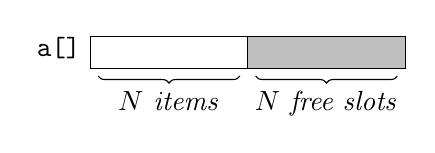
\begin{tikzpicture}
    \draw (0,0) 
          node[anchor=south east] {\texttt{a[]}}
          rectangle (2,.4);
    \draw [fill=gray!50] (2,0) rectangle (4,.4);
    \draw (1.9,-.1)[decorate, decoration=brace]
          -- node[below=2pt] {\textit{$N$ items}}
          (.1,-.1);
    \draw (3.9,-.1)[decorate, decoration=brace] 
          -- node[below=2pt] {\textit{$N$ free slots}} 
          (2.1,-.1);
  \end{tikzpicture}
  \caption{The data structure immediately after {\tt resize()}.}
\end{marginfigure}



With this observation, we can proceed to show that at the start of
every subsequent call of {\tt resize()}, there are at least $4N$ coins
in the bank.
\begin{itemize}
\item If the call came from \texttt{push()}, i.e., to prevent
  overflow, then there must have been at least $N/2$ calls to
  \texttt{push()} since the last \texttt{resize()}. Each
  \texttt{push()} deposited 8 coins, so there are $4N$ coins, as
  needed.
\begin{marginfigure}
  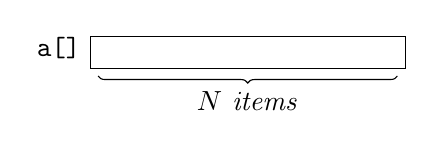
\begin{tikzpicture}
    \draw (0,0) 
          node[anchor=south east] {\texttt{a[]}}
          rectangle (4,.4);
    \draw (3.9,-.1)[decorate, decoration=brace]
          -- node[below=2pt] {\textit{$N$ items}}
          (.1,-.1);
  \end{tikzpicture}
  \caption{The data structure immediately before \texttt{push()} calls
    \texttt{resize()}.}
\end{marginfigure}
\item If the call came from \texttt{pop()}, i.e., to prevent underflow,
  then there must have been at least $N$ calls to \texttt{pop()} since
  the last \texttt{resize()}. Each \texttt{pop()} deposited 4 coins,
  so there are $4N$ coins, as needed.
\begin{marginfigure}
  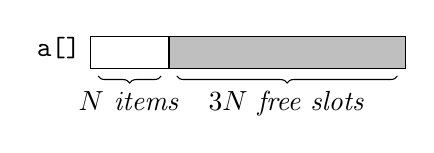
\begin{tikzpicture}
    \draw (0,0) 
          node[anchor=south east] {\texttt{a[]}}
          rectangle (1,.4);
    \draw [fill=gray!50] (1,0) rectangle (4,.4);
    \draw (0.9,-.1)[decorate, decoration=brace]
          -- node[below=2pt] {\textit{$N$ items}}
          (.1,-.1);
    \draw (3.9,-.1)[decorate, decoration=brace] 
          -- node[below=2pt] {\textit{$3N$ free slots}} 
          (1.1,-.1);
  \end{tikzpicture}
  \caption{The data structure immediately before \texttt{pop()} calls {\tt resize()}.}
\end{marginfigure}
\end{itemize}
This finishes the proof of proposition E.

\begin{ExerciseList}
  \Exercise Can we charge all costs to
  \texttt{push()}? How much does it have to pay if \texttt{pop()} pays nothing?
  \Exercise Can we charge all costs to
  \texttt{pop()}? How much does it have to pay if \texttt{push()} pays nothing?
\end{ExerciseList}

\subsection{Localising the piggy bank argument}

Sometimes it is easier to localise the accounting argument by removing
the fictional piggy bank and depositing the coins in the data
structure instead.

For example, we can say that push operation puts 8 coins in the cell
it just filled, and every pop puts 4 coins in the cell that it just
freed. 

As before, when doubling the array from $N$ to $2N$, we argue that at
least $N$ {\tt push()} operations happened, so the entries in {\tt a}
from $N/2-1$ to $N$ contain at east 8 coins each, for a total of $4N$
coins. Similarly, for halving the array from $4N$ to $2N$, the calls
to {\tt pop()} put 4 coins on each of the free cells in $N+1,\ldots,
2N$, for a total of $4N$ coins. 

The local argument is sometimes attractive because there is a strong
inuition about what the coins will be doing, should they ever be
needed.  
For example, the 4 coins deposited by {\tt push} in position {\tt
  a[N+1]} will be able to pay for the allocation of the new array
cells {\tt temp[1]} and {\tt temp[N+1]}, and the two accesses in {\tt
  temp[1] = a[1]}.

\begin{marginfigure}
 %  \begin{tikzpicture}[font=\tt,scale=.4]
%     \draw (0,0)
%           node[anchor=south east] {\texttt{a[]}}
%           rectangle (.4,.4) ;
%     \node (pop1) at (0,-1) [anchor=west] {pop()};
%     \draw (0,-2)
%           node[anchor=south east] {\texttt{a[]}};
%           \matrix[every node/.style={draw,inner sep=0pt,
%             minimum height=8pt, minimum width=15pt},
%           matrix of nodes,nodes in empty cells] {
%            to & be & or & not
%             &|[gray]|\textrm{\it null}
%             &\textrm{\it null}
%             &\textrm{\it null}
%             &\textrm{\it null}\\
%           };
%           grid +(8,1);
%     \node (pop2) [below of= pop1, anchor=west] {pop()};
%     \node (pop3) [below of= pop2, anchor=west] {pop()};
%   \end{tikzpicture}
% %
\tikzstyle{cell}=[draw,on chain,minimum width=6mm,
  font=\tiny\tt, text height=1.25ex, text depth=.25ex]
\tikzstyle{coin}=[draw,circle, inner sep= 1pt, fill=white,font=\tiny\sf]
\begin{tikzpicture}
\begin{scope}[start chain, node distance=0cm]
  \node[on chain] {\tt\textcolor{red} a};
  \foreach \word in {to, be, or, not} \node [cell]{\word};
  \foreach \i in {4,...,7} \node [cell] {\it null};
\end{scope}
\node at (0,-1) [anchor=west]{\tt pop(); pop();} ;
\begin{scope}[start chain, node distance=0cm]
  \node at (0,-2) [on chain] {\tt\textcolor{red} a};
  \foreach \word in {to, be} \node (a\word) [cell]{\word};
  \foreach \i in {2,...,7} \node [cell](C\i) {\it null};
\end{scope}
\begin{scope}[start chain= going {at=(\tikzchainprevious),shift=(-40:.2)},node distance=0cm]
\node (R2) [on chain,below of=C2, coin] {R};
\node (W2) [on chain, coin] {W};
\node (N21) [on chain, coin] {N};
\node (N22) [on chain, coin] {N};
\end{scope}
\begin{scope}[start chain= going {at=(\tikzchainprevious),shift=(-40:.2)},node distance=0cm]
\node (R3) [on chain,below of=C3, coin] {R};
\node (W3) [on chain, coin] {W};
\node (N31) [on chain, coin] {N};
\node (N32) [on chain, coin] {N};
\end{scope}
\node at (0,-3) [anchor=west]{\tt Item[] temp = (Item []) new
  Object[4]};
\begin{scope}[start chain, node distance=0cm]
  \node at (0,-4) [on chain] {\tt\textcolor{red} temp};
  \foreach \i in {0,...,3} \node (NN\i) [cell] {\it null};
\end{scope}
\node at (0,-5) [anchor=west]{\tt temp[0] = a[0]; temp[1] = a[1]; };
\begin{scope}[start chain, node distance=0cm]
  \node at (0,-6) [on chain] {\tt\textcolor{red} temp};
  \node (to) [cell] {to};   \node (be) [cell] {be};
  \foreach \i in {2,...,3} \node [cell] {\it null};
\end{scope}
\draw [->,nearly transparent] (N21) to[out=270,in=90] (NN0);
\draw [->,nearly transparent] (N22) to[out=270,in=90] (NN1);
\draw [->,nearly transparent] (N31) to[out=270,in=90] (NN2);
\draw [->,nearly transparent] (N32) to[out=270,in=90] (NN3);
\draw [->,nearly transparent] (R2) to[out=270,in=270] (ato);
\draw [->,nearly transparent] (R3) to[out=270,in=270] (abe);
\draw [->,nearly transparent] (W2) to[out=270,in=90] (to);
\draw [->,nearly transparent] (W3) to[out=270,in=90] (be);
\end{tikzpicture}
%
\caption{
  Two pop operations each deposit 4 coins (marked N, N, R, W), in
  {\tt a[2]} and {\tt a[3]} respectively.
  When {\tt resize()} is called, the coins
  marked N are spent allocated the new array {\tt temp}, the R coin is
  spent reading from {\tt a}, and the W coin is spent writing to {\tt
    temp}. In the new {\tt a} (which is {\tt temp}), there is no money.
}
\end{marginfigure}

But it's a matter of taste. I like the local argument better for
exercise~X.



\section{Mechanical Counter}

Whenever a mechanical counter is incremented, the rightmost wheel (the
``ones'') is turned. Every 10th increment, when the rightmost wheel
transitions from 9 to 0, its left neighbour is turned as well. This
effect continues to the left, so after $10^k-1$ increments, when the
counter shows $k$ 9s, the next increment will lead $k+1$ wheels to
turn.

\begin{figure}[htb]
\centerline{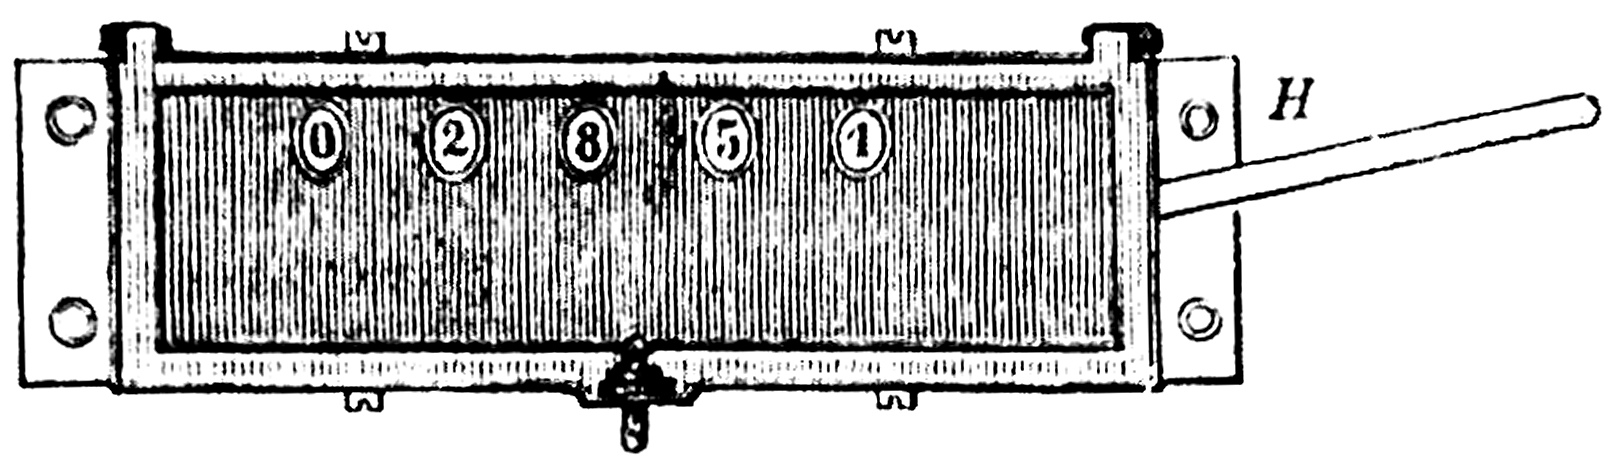
\includegraphics[width=2in]{Zaehlwerk_Schema_1.jpg}
$\quad$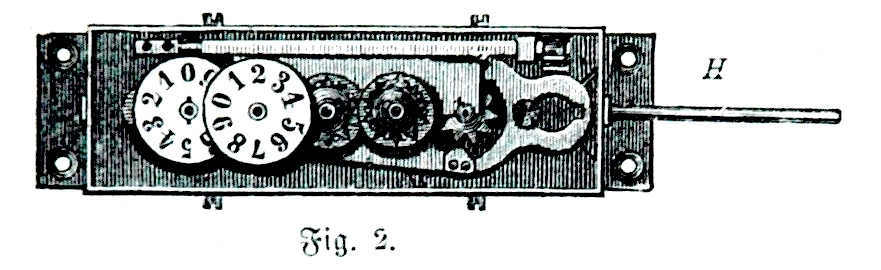
\includegraphics[width=2in]{Zaehlwerk_Schema_2_clean.png}}
\caption{A 5-digit mechanical counter.}
\end{figure}

In our terminology, the worst case number of operations for $N$
increments is logarithmic. But in the amortised sense, the behaviour
is much better:

\begin{quote}
  {\bf Proposition C.}  Starting from 0, a mechanical counter needs a
  constant amortised number of operations per increment.
\end{quote}

To establish this, we can use the ``easy'' aggregate method. Let
$N\geq 0$
be the total number of increments, and let us look at each wheel
separately. Number then $0,\ldots, k-1$ from right to left, so wheel~$0$
are the ones and $k=\lfloor \log_{10} N\rfloor$.

Wheel $0$ was rotated $N$ times. Wheel $1$ was rotated $\lfloor
N/10\rfloor$ times. In general, wheel $r$ was turned \[ \left \lfloor
\frac{N}{10^r} \right\rfloor\] times ($0\leq r < k$). Summing these
contributions for the total number of operations, gives 
\begin{multline*}
 \left \lfloor
\frac{N}{10^0} \right\rfloor +
 \left \lfloor
\frac{N}{10^1} \right\rfloor +
\cdots +
 \left \lfloor
\frac{N}{10^{k-1}} \right\rfloor
\leq \\
\frac{N}{10^0} +
\frac{N}{10^1} +
\cdots +
\frac{N}{10^{k-1}} 
=
N\left(\frac{1}{10^0}+\frac{1}{10^1}+\cdots+\frac{1}{10^{k-1}} \right)
< 2N.
\end{multline*}
This finishes the proof.

\begin{ExerciseList}
\Exercise
Prove proposition~C using the piggy bank method instead.
If you use the local argument, where does the money go?
How little do you actually need?
\footnote{To make this entertaining, assume it takes one pound
  sterling to turn a wheel and give the answer in pence.
  Next, assume it takes 1 shilling.}
\Exercise
 Assume the counter is built out of increasingly heavy material. 
 Each wheel costs twice as much to turn as the previous.
 (So, turning wheel 0 costs 1, wheel 1 costs 2, wheel 2 costs 4, 
 $\ldots$,  wheel $k$ costs $2^k$.)
 Does the analysis still work?
 What if wheel $k$ costs $10^k$? $11^k$?
\end{ExerciseList}

\section{Weighted quick-find}

\emph{This makes sense after [SW] 1.5}

\bigskip
We return to the first, very simple union-find data structure of [SW],
called \emph{quick-find}. 

Let us try to salvage this idea, at least partially. We're not going
to be able to beat the quick-union implementations, but this section
is mainly about \emph{analysis}, not so much about giving the best
union--find algorithm known to Man.

Our first improvement is to make a clever choice about whether
\texttt{union(p, q)} renames {\tt p}'s component to {\tt q}'s or vice
versa. 
Our choice is to always rename the smaller component.
For this, we introduce another array {\tt int[] sz} to store component
sizes, initially all $1$, and with the same meaning as in
algorithm~1.4.

The second improvement is to link all elements of a component, so that
we can quickly iterate over them when we want to rename them, instead
of iterating over all of {\tt id}.
For this, we implement yet another array {\tt int[] next} of indices,
so that {\tt next[i]} is the element following {\tt i} in some
circular list of the component ids.

For example, the data structure looks like this after the operations
described by {\tt tinyUF.txt}.:

\medskip
{\tt \small
  \begin{tabular}{rcccccccccc}
      & 0 & 1 & 2 & 3 & 4 & 5 & 6 & 7 & 8 & 9 \\\midrule
id[] & 6 &6 &6 &4 &4 &6 &6 &6 &4 &4 \\
next[] & 5 &2 &0 &4 &9 &6 &7 &1 &3 &8 \\
sz[] &1 &1 &3 &1 &4 &1 &6 &1 &1 &1 
  \end{tabular}}
\medskip

Figure \ref{fig: WUF} shows the this situation, and the situation
after another call to {\tt union()}. 
An implementation is given in figure~\ref{fig: WUF impl}.

\begin{marginfigure}
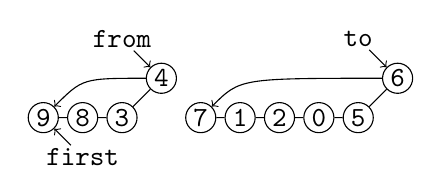
\begin{tikzpicture}[font=\tt,scale=.5,every node/.style={draw,circle,
    inner sep=1pt}]
  \node (9) at (0,0) {9};
  \node (8) at (1,0) {8};
  \node (3) at (2,0) {3};
  \node (4) at (3,1) {4};

  \node (7) at (4,0) {7};
  \node (1) at (5,0) {1};
  \node (2) at (6,0) {2};
  \node (0) at (7,0) {0};
  \node (5) at (8,0) {5};
  \node (6) at (9,1) {6};
  \draw[->] (7)--(1)--(2)--(0)--(5)--(6).. controls(5,1)..(7);
  \draw[->] (9)--(8)--(3)--(4)..controls(1,1)..(9);

  \node[draw=none,rectangle] at (1,-1) {first} edge [->] (9);
  \node[draw=none,rectangle] at (2,2) {from} edge [->] (4);
  \node[draw=none,rectangle] at (8,2) {to} edge [->] (6);
\end{tikzpicture}

\bigskip
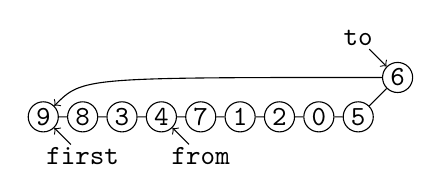
\begin{tikzpicture}[font=\tt,scale=.5,every node/.style={draw,circle,
    inner sep=1pt}]
  \node (9) at (0,0) {9};
  \node (8) at (1,0) {8};
  \node (3) at (2,0) {3};
  \node (4) at (3,0) {4};

  \node (7) at (4,0) {7};
  \node (1) at (5,0) {1};
  \node (2) at (6,0) {2};
  \node (0) at (7,0) {0};
  \node (5) at (8,0) {5};
  \node (6) at (9,1) {6};
  \draw[->]   (9)--(8)--(3)--(4)--(7)--(1)--(2)--(0)--(5)--(6)
  ..controls(1,1)..(9);

  \node[draw=none,rectangle] at (1,-1) {first} edge [->] (9);
  \node[draw=none,rectangle] at (4,-1) {from} edge [->] (4);
  \node[draw=none,rectangle] at (8,2) {to} edge [->] (6);
\end{tikzpicture}
\bigskip
\caption{\label{fig: WUF}{\tt union(1,8)}, where {\tt id[8] == 4} and {\tt id[1] ==
    6}.  The {\tt next} pointers are shown.}
\end{marginfigure}


\begin{figure}
\begin{tikzpicture}[remember picture,overlay] 
  \draw [fill=orange!30]
  (current page.south west) rectangle (current page.north east); 
\end{tikzpicture}

Algorithm A.1 Weighted quick-find implementation

\small
\begin{lstlisting}[basicstyle=\ttfamily,backgroundcolor=\color{white},
  frame=single,rulecolor=\color{gray!20},framesep=10pt, linewidth=12cm]
public class WeightedQuickFind
{
  private int[] id, sz, next;
  private int count;

  public WeightedQuickFind(int N)
  {
    count = N;
    id = new int[N];
    next = new int[N];
    sz = new int[N];
    for (int i = 0; i < N; i++) 
    { 
      id[i] = i;
      next[i] = i;
      sz[i] = 1;
    }
  }

  private void rename(int from, int to)
  {
    int first = next[from];
    for (int i = first; i != from; i = next[i])
	id[i] = to;
    id[from] = to;
    next[from] = next[to];
    next[to] = first;
    sz[to] += sz[from];
  }

  public void union(int p, int q) 
  {
    int pID = find(p); 
    int qID = find(q);
    if (pID == qID) return;
    if (sz[pID] < sz[qID]) rename(pID,qID);
    else                   rename(qID,pID);
    count--;
  }
  \\ see [SW], sect. 1.5 for find, count, connected, main
}
\end{lstlisting}
\caption{\label{fig: WUF impl}Weighted quick-find.}
\end{figure}

It is easy to construct a sequence of {\tt union()} operations that
result in linear worst-case time per operation. (Construct such a
sequence.) However, we show that in the amortised sense, the data
structure is pretty fast:

\begin{quote}
  {\bf Proposition A4.} In the weighted quick-find implementation, any
  sequences of {\tt union()} operations takes amortized logarithmic
  time in the worst case.
\end{quote}

We can show this using the aggregate method, so we consider a sequence
of $k$ calls to {\tt union()}.

We will count the number of updates of {\tt id[]} in {\tt rename()},
from the perspective of a single site $i$. 
The crucial observation is that whenever the {\tt id} of $i$ is
renamed, the size of its component at least doubles.
(This is because we always rename the smaller of two unioned
components, and the size of the union is at least twice of the smaller
one.)
On the other hand, no component can ever be larger than $k+1$. 
(This is because every elemented started out in a component of its
own.
At some time, this component must have been united with the others,
which must have required a call to {\tt union()}.)
Thus, no component can have been doubled more than $\log (k+1)$ times.
In particular, the {\tt id[i]} has been renamed at most $\log
(k+1)$ times.

We are close to finishing the argument and tempted to say ``since
there are $N$ sites, and we just saw that each gets renamed $~\log k$
times in total during the $k$ operations, so the amortised time per
operation is $N\log k / k$, so --- hmmm $\ldots$.''

We need one more observation: if site $i$ does not occur as an
argument to {\tt union()} during the $k$ operations, then it is never
renamed. Thus, at most $2k$ sites are ever renamed. Now we an finish:
Since only $2k$ sites are ever renamed, and we just saw that each site
gets renamed at most $\sim\log k$ times in total, there are $\sim
2k\log k$ array updates. Thus the amortised time per operation is
$\sim 2k\log k / k = 2\log k$, i.e., logarithmic in $k$. This finishes
the proof of propostion A4.

\section{A Dictionary of Sorted Lists}

[TODO]

\end{document}
